% Created 2020-05-06 mié 13:45
% Intended LaTeX compiler: pdflatex
\documentclass[a4paper, 12pt]{article}
\usepackage[utf8]{inputenc}
\usepackage[T1]{fontenc}
\usepackage{graphicx}
\usepackage{grffile}
\usepackage{longtable}
\usepackage{wrapfig}
\usepackage{rotating}
\usepackage[normalem]{ulem}
\usepackage{amsmath}
\usepackage{textcomp}
\usepackage{amssymb}
\usepackage{capt-of}
\usepackage{hyperref}
\usepackage{float, amsfonts, commath, mathtools}
\author{Tabaré Pérez}
\date{\today}
\title{Lecture 13 - 4: Another Clustering Example: Image Quantization}
\hypersetup{
 pdfauthor={Tabaré Pérez},
 pdftitle={Lecture 13 - 4: Another Clustering Example: Image Quantization},
 pdfkeywords={},
 pdfsubject={},
 pdfcreator={Emacs 26.3 (Org mode 9.3.6)}, 
 pdflang={English}}
\begin{document}

\maketitle
So Google News example is an example of use of clustering for visualization.
Let's look at a very different application of clustering and this time for data
compression. So the specific application that I will talk about is called:

IMAGE QUANTIZATION

So let's assume that a typical picture would have 1,024 by 1024 pixels. Now,
each pixel is encoded by 24 bits because you have 8 bits for red, 8 bits for
blue, and 8 beads for green. So therefore a typical image would be the number of
pixel multiplied by the number of bits we need to store each pixel:

\begin{itemize}
\item red - 8 bits
\item green - 8 bits
\item blue - 8 bits
\end{itemize}

\begin{equation} 
1024 \times 1024 \times 24 = \text{3Mb}
\end{equation}

Let's say I want to compress it and to use much less space to get high-quality
image.

So one option for me is to say that instead of using such a rich representation
of the pixel I am going to greatly limit myself: I will just allow myself, let's
say, to have 32 colors.

First of all, 32 colors is not that bad, but let's say we are just limited to
use only 32 colors. In this case, we would need only two \(2^5\) (5 bits) to
encode them, which makes it much easier.

So now if we are looking at the same pictures that we had before, we will have
1,024 by 1,024 pixels, and then each one of them would be just represented by 5
bits.

In addition, we also would need to store the dictionary which remember how
we can translate each one of these colors to our original encoding in this
24-bit representation.

So again, this part will be just representing every pixel by 1 of 32 colors, and
this part would remember how to translate our colors that we selected in the
encoding of the 24 bits, which was original encoding of our pixel. In this
case, we would have much smaller representation of the image.

\begin{equation}
1024 \times 1024 \times 5 + 32 \times 24 = \text{640Kb}
 \end{equation}

So the question that you may be asking yourself, now I started with looking
at this very high-resolution image where we can encode so many different colors,
and I limited myself just to a few colors: How well does it work?

So let's take a look at a concrete picture and see how this process actually
reflects on the picture quality.

\begin{figure}[H]
\centering
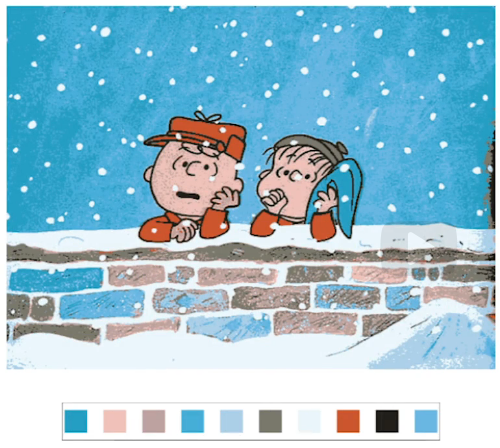
\includegraphics[width=0.5\textwidth]{./pic/cartoon-01.png}
\caption{\label{fig:org14b1427}24 bits color image}
\end{figure}

So here you can see an image from a cartoon, and it uses quite a number of
colors. And if you remember how the pixel is represented, in theory we can have
\(2^{24}\) different colors.

So now I will go to an extreme. And instead of using so many different colors, I
would allow you to use just two colors.

\begin{figure}[H]
\centering
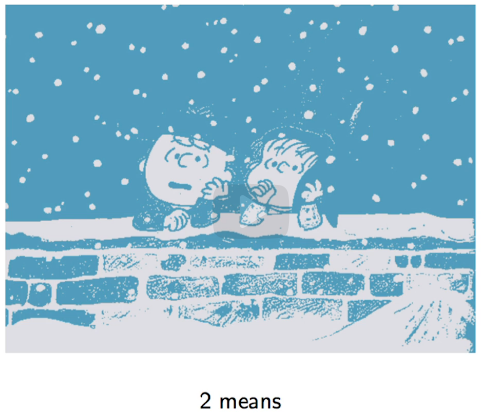
\includegraphics[width=0.5\textwidth]{./pic/cartoon-02.png}
\caption{\label{fig:org723004c}2 colors}
\end{figure}

And in this case, we can see this image represented with two colors. Obviously
we lose most of the details but we can still recognize the characters. We will
get great compression rate but will clearly negatively impact the quality of the
picture.

Now, I would give you a bit more colors and allow you to use four.

\begin{figure}[H]
\centering
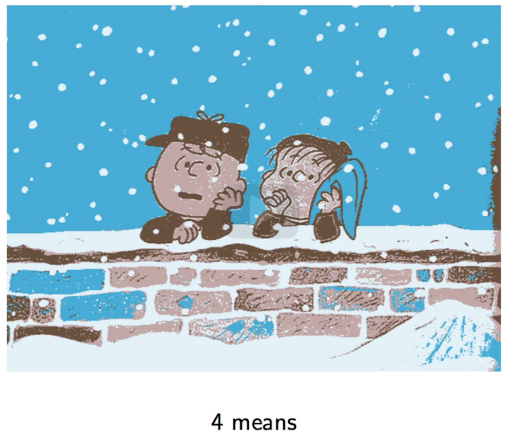
\includegraphics[width=0.5\textwidth]{./pic/cartoon-03.png}
\caption{\label{fig:org436a168}4 colors}
\end{figure}

In this case, it already looks a lot like a real cartoon, but we can still see
that there is a big difference in resolution between the original image and this
particular one.

However, as we continue to increase the number of colors, for instance here we
have 16 colors,

\begin{figure}[H]
\centering
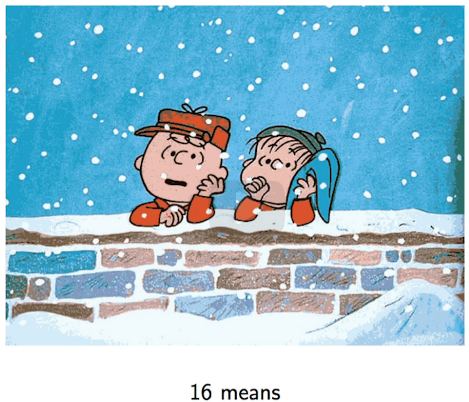
\includegraphics[width=0.5\textwidth]{./pic/cartoon-04.png}
\caption{\label{fig:orgd4c8e45}16 colors}
\end{figure}

we can clearly see that this image looks so much better, and it looks very close
to the original image.

Now if I would use 32 colors, as the example that I showed you on the board
previously, here I would say that for untrained observer, it will be almost
impossible to distinguish this image from the original image.

\begin{figure}[H]
\centering
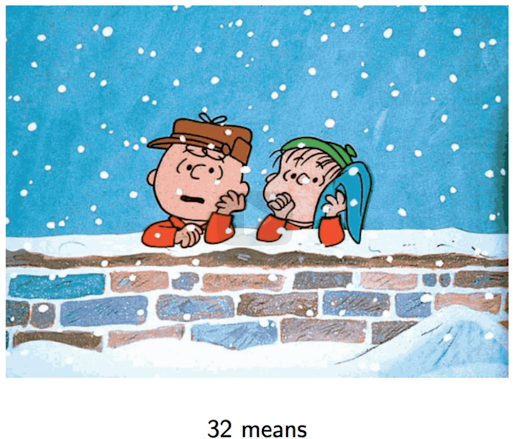
\includegraphics[width=0.5\textwidth]{./pic/cartoon-05.png}
\caption{\label{fig:org68ee0af}32 colors}
\end{figure}

So here we can say that we really hit a sweet spot between compressing the image
but at the same time preserving the quality of the color of the image.

I will continue, I would show you 64 colors:
\begin{figure}[H]
\centering
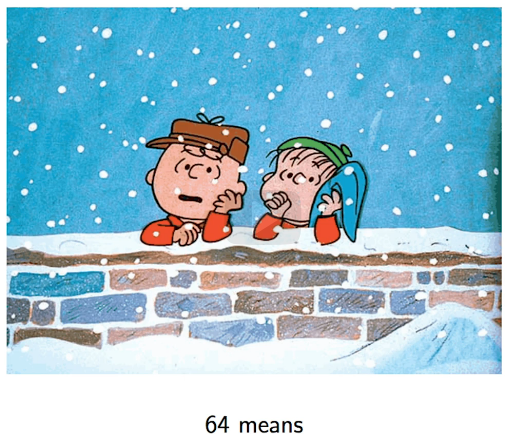
\includegraphics[width=0.5\textwidth]{./pic/cartoon-06.png}
\caption{\label{fig:orge025ef3}64 colors}
\end{figure}

Again, it's even more precise.

And finally in 128 colors, we clearly will be unable by human eye to distinguish
this picture from the original painting.

\begin{figure}[H]
\centering
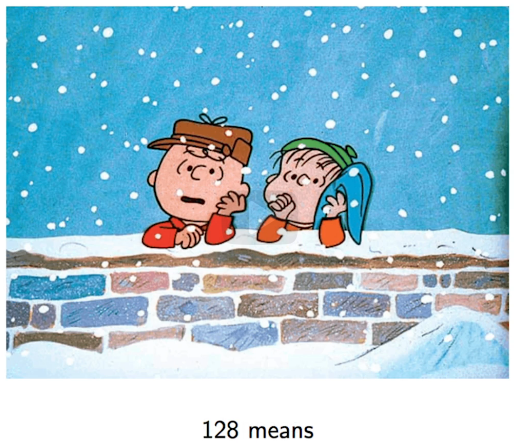
\includegraphics[width=0.5\textwidth]{./pic/cartoon-07.png}
\caption{\label{fig:orgb1e08ad}128 colors}
\end{figure}

But what this progression between the number of clusters, the compression rate,
and the quality brings us a very important point about the number of clusters
and the impact on the resulting quality because here we have two contrasting
goals:

\begin{itemize}
\item One goal is to make our image as compressed as possible.
\item The second goal is obviously to preserve the quality.
\end{itemize}

And you have control over it by deciding how many clusters do you have, and it
will depend on your space requirement, on your output requirement, and so on. As
a developer, you can decide what is your perfect number of clusters K should be.

So now I concluded the description of this example, and I want to bring to your
attention these two examples of clustering that we've seen:

\begin{itemize}
\item Google News visualization.
\item Image quantification.
\end{itemize}

In both of these examples, we went through the same process.

\begin{enumerate}
\item We started by taking our instances and representing them as vectors:

\begin{itemize}
\item In the case of Google News, it was stories that we translated using bag of
words into a vector.
\item In teh case of the image, it was a pixel which we had represented as a
vector of 24 bits.
\end{itemize}

\item The second step for us was to find a similarity measure which can compare
between these two vectors.

\item And finally, we would use some clustering algorithm which would tell us how to
group them.
\end{enumerate}

So in this case, for instance, after we finished the grouping, we will select
one representative color for the cluster and use them in the picture.

In the case of Google News, we selected one representative story to show as a
central story in the news.
\end{document}